% 第一版:晚来秋 小红书号:4475058927
% 第二版:失去理想的环 小红书号:9650811380
% 转载请注明出处!

\documentclass[12pt]{article}
\usepackage{pst-poker}           % 提供扑克牌点数、花色符号
\usepackage[poster]{tcolorbox}   % 用于tcbposter分块布局
\usepackage[papersize={5.7cm,8.8cm}]{geometry} % 设置纸张尺寸(类似扑克牌)
\usepackage{amssymb, bm, graphicx, hyperref, mathrsfs,geometry,xcolor,color}

\pagestyle{empty} % 隐藏页码等页面样式


\begin{document}

\begin{tcbposter}[
    poster = {columns=130, rows=150, spacing=0mm}, % 划分130列150行,间距0
    coverage = {spread, left=0.1cm, right=0.1cm, top=0.1cm, bottom=0.1cm}, % 页面边距
    boxes = {
        boxrule=0mm,    % 默认框线宽度
        colback=white,  % 背景色
        colframe=white, % 框线颜色
        left=0mm, right=0mm, top=0mm, bottom=0mm % 内边距
    },
]
% 1. 绘制扑克牌外边框
\posterbox[
    boxrule=0.5mm,     % 边框宽度
    colback=white,     % 背景色
    colframe=black!80, % 边框颜色(黑灰色)
]{name=border, row=1, column=1, span=130, rowspan=150}{} % 跨130列150行,作为外框

% 2. 左上角:点数 + 花色
\posterbox[
    valign=top,    % 垂直对齐:顶部
    halign=left,   % 水平对齐:左侧
    boxrule=0mm,   % 框线宽度0
    colback=white, % 背景色
]{name=top-left, row=5, column=4, span=1, rowspan=1}{
  {\huge \psset{inline=symbol} \Qh } % 示例:红桃Q
}

% 2.1 上半部分靠左插入正向图片
\posterbox[
    valign=top,    % 垂直对齐:顶部
    halign=left,   % 水平对齐:左侧
    boxrule=0mm,   % 框线宽度0
    colback=white, % 背景色
]{name=top-image, row=25, column=15, span=60, rowspan=40}{%
  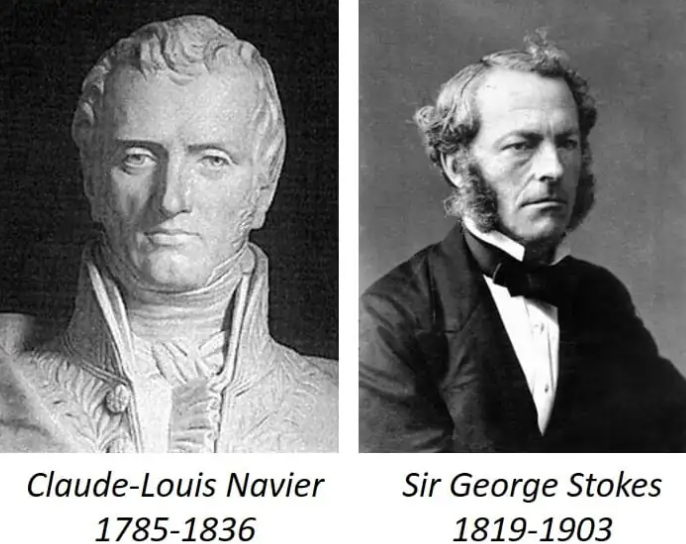
\includegraphics[width=\linewidth, height=3cm, keepaspectratio]{头像2.png} % 替换为你的图片路径
}

% 2.2 上半部分靠右插入文字
\posterbox[
    valign=top,    % 垂直对齐:顶部(上半部分)
    halign=right,   % 水平对齐:右侧
    boxrule=0mm,
    colback=white,
]{name=top-char, row=20, column=90, span=15, rowspan=45}{% 位置:右上区域,占据足够高度
  \rotatebox{270}{% 旋转270°实现“从上至下”竖排
    {\fontsize{20}{24}\selectfont Analysis} % 行书字体,字号20pt
  }
}

% 3. 中间区域:数学公式
\posterbox[
    boxrule=0mm,     % 框线宽度0
    frame hidden,    % 隐藏框线
    halign=center,   % 水平居中
    valign=center,   % 垂直居中
]{name=middle, row=74, column=2, span=127, rowspan=2}{
  {\fontsize{5.5}{0}\selectfont
    $$
    \rho \left( \frac{\partial \boldsymbol{u}}{\partial t} + (\boldsymbol{u} \cdot \nabla) \boldsymbol{u} \right) = -\nabla p + \mu \nabla^2 \boldsymbol{u} + \rho \boldsymbol{f}
    $$
  }
}

% 4.1 下半部分靠右插入旋转180°的图片
\posterbox[
    valign=bottom,  % 垂直对齐:底部
    halign=right,   % 水平对齐:右侧
    boxrule=0mm,    % 框线宽度0
    colback=white,  % 背景色
]{name=bottom-image, row=90, column=54, span=60, rowspan=40}{%
  \rotatebox{180}{% 旋转180度
    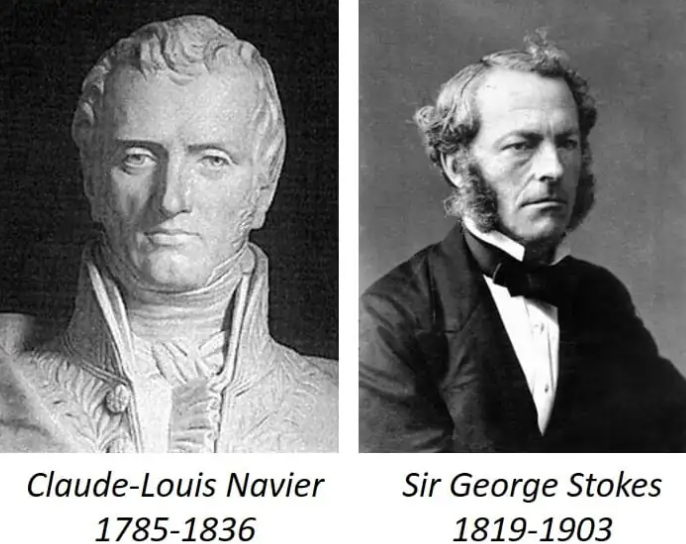
\includegraphics[width=\linewidth, height=3cm, keepaspectratio]{头像2.png} % 替换为你的图片路径
  }
}

% 4.2 下半部分
\posterbox[
    valign=top,    % 垂直对齐:顶部(上半部分)
    halign=right,   % 水平对齐:右侧
    boxrule=0mm,
    colback=white,
]{name=top-char, row=88, column=23, span=15, rowspan=45}{% 位置:右上区域,占据足够高度
  \rotatebox{90}{% 旋转90°实现“从上至下”竖排
    {\fontsize{20}{24}\selectfont Analysis} % 行书字体,字号20pt
  }
}

% 4. 右下角:点数 + 花色(旋转180°,与左上角对称)
\posterbox[
    boxrule=0mm,   % 框线宽度0
    halign=right,  % 水平对齐:右侧
    valign=bottom, % 垂直对齐:底部
    colback=white, % 背景色
]{name=bottom-right, row=146, column=90, span=1, rowspan=1}{
  \rotatebox{180}{% 旋转180度
    {\huge \psset{inline=symbol} \Qh}
  }
}

\end{tcbposter}
\end{document}